% Figure 1: Draphnet schematic
\begin{figure}[htbp]
\centering

\includegraphics[width=0.85\textwidth]{figures/fig_schematic.pdf}
\caption{Draphnet integrates three input matrices into a single logistic
affinity-regression model. The drug-by-endpoint matrix $D$ (429 compounds
$\times$ 1391 ToxCast endpoints) is dimensionality-reduced via SoftImpute
to $U_D S_D$; the gene-by-phenotype matrix $P$ (10,027 genes $\times$ 197
UK Biobank phenotypes from PhenomeXcan) is reduced via singular-value
decomposition; and a shared interaction matrix $W_{DP}$ is trained by
$L_1$-regularized logistic regression to predict the binary drug-phenotype
annotation matrix $Y$ from SIDER.}
\label{fig:schematic}
\end{figure}

% Figure 2: prediction performance
\begin{figure}[htbp]
\centering
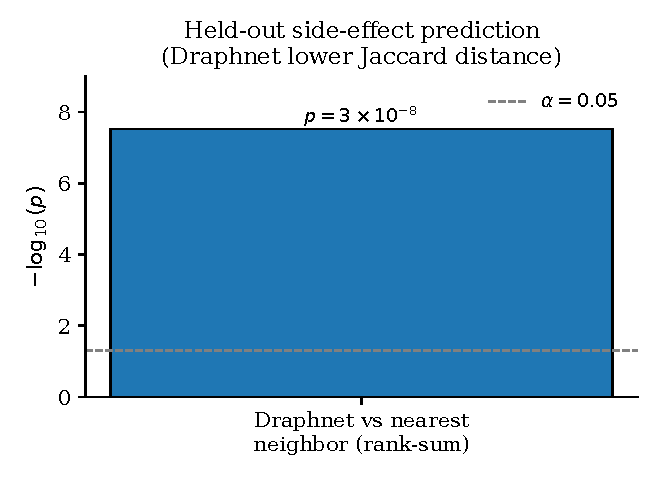
\includegraphics[width=0.55\textwidth]{figures/fig_prediction.pdf}
\caption{Held-out side-effect prediction. On a 20-fold cross-validation over
drugs (5\% held out per fold), Draphnet produces lower Jaccard distance
between predicted and observed SIDER profiles than a nearest-neighbor
baseline trained in the same $D$ space (rank-sum $p=3\times 10^{-8}$).
Dashed line marks the $\alpha=0.05$ significance threshold.}
\label{fig:prediction}
\end{figure}

% Figure 3: target-level enrichment
\begin{figure}[htbp]
\centering
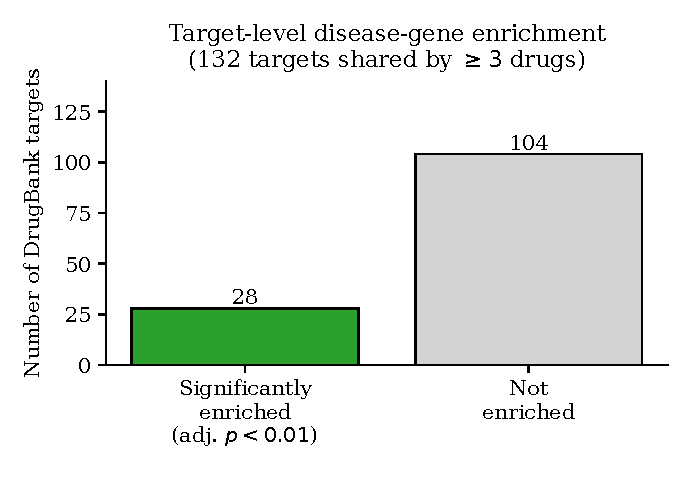
\includegraphics[width=0.55\textwidth]{figures/fig_enrichment.pdf}
\caption{Target-level enrichment of disease-gene associations. Of 132
DrugBank targets that are shared by at least three drugs in our set, 28
($21\%$) have one or more disease genes significantly associated with
drug-target membership at Benjamini-Hochberg-adjusted $p<0.01$ (the
empirical permutation null is illustrated in Fig.~3A of the Results text).}
\label{fig:enrichment}
\end{figure}

% Figure 4: highlighted drug-gene associations (placeholder)
\begin{figure}[htbp]
\centering
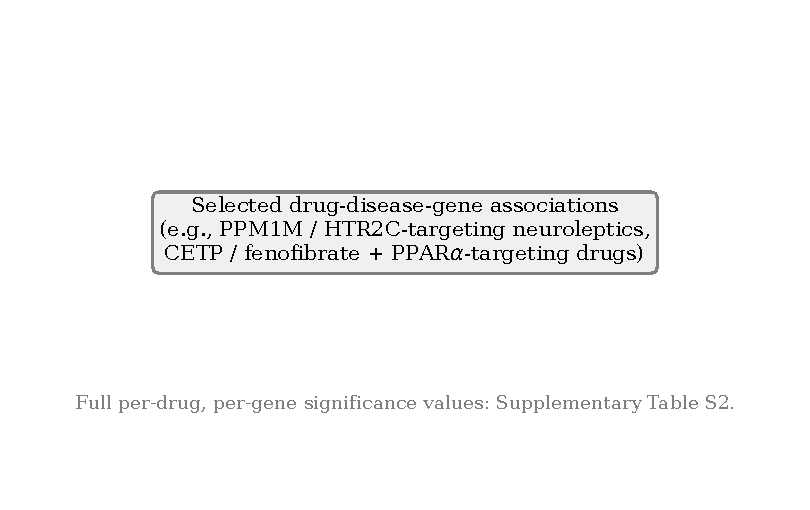
\includegraphics[width=0.7\textwidth]{figures/fig_associations.pdf}
\caption{Representative drug-disease-gene associations identified by
Draphnet, including PPM1M for HTR2C-targeting neuroleptics and CETP for
fenofibrate and other PPAR$\alpha$-targeting drugs. Per-drug significance
values are provided in Supplementary Table S2; this figure summarizes the
categories discussed in the Results.}
\label{fig:associations}
\end{figure}
